\pagestyle{fancy}

\graphicspath{ {Figures/Chapter4_IntensitySimulation/} }

In this chapter, the signal generation in secondary emission monitors (SEM) when traversed by a particle beam will be covered. The formulations are going to be rather broad, for a generic particle beam and energy range. However, all the numerical examples will refer to SEM grids and Wire Scanner detectors in LINAC4. 

\section{Signal Generation in SEM}

At first, one can define the net charge generated on a wire or a foil transversed by a particle projectile (Proj) as: 

\begin{equation}
    \label{eq:Qsum}
    Q\left(\frac{e}{Proj}\right) = Q_{dep} + Q_{SE} + Q_{th}
\end{equation}

Where $Q_{dep}$ represents the charge genration due to Charge deposition. $Q_{SE}$ is the charge due to secondary emission and $Q_{th}$ is the charge due to thermionic emission. Figure \ref{fig:SignalGeneration} shows a schematic representation of the different processes that contribute to the charge generation in the material. They will be detaidely covered in the next sections. 

\begin{figure}[h]
    \centering
    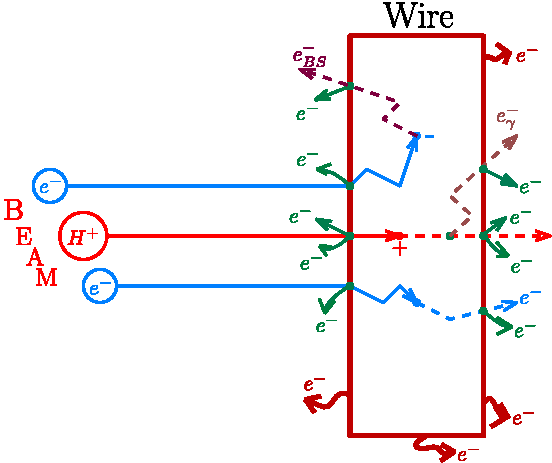
\includegraphics[width=0.50\columnwidth]{Figure_ChargeGeneration/ChargeGen.pdf}
    \caption{Schematic Representation of processes inducing current in the detector material.}
    \label{fig:SignalGeneration}
\end{figure}

\subsection{Charge Deposition ($Q_{dep}$)}

When an ion with $N_p$ number of protons in the nucleus and $N_e$ non-stripped electrons hits a target, the electrical charge directly deposited in the target depends on the probability of the protons and the electrons remaining on it. This can be written as: 

\begin{equation}
    Q_{dep} = N_p \cdot \eta - N_{e}\cdot \mu
\end{equation}

Where $\eta$ is the proportion of protons that are stopped in the material and $\mu$ is the proportion of electrons. These parameters depend on the range of the particles in the detector material, which was described in \ref{sec:Range}, and on the back-scattering probability, explained in \ref{sec:BS}. 

\subsection{Secondary Emission Charge ($Q_{SE}$)} 

The charge generated in the material by a particle, with $N_p$ number of protons and $N_e$ number of electrons, can be modeled as: 

\begin{equation}
    \begin{split}
        Q_{SE} = N_p \cdot SEY_{p1} + N_p \left(1-\eta\right)SEY_{p2} + 
                N_e \cdot SEY_{e1} + N_e \left( 1 - \mu \right) SEY_{e2} + \\
                N_p \cdot BS_p \cdot SEY_{BSp} + N_e \cdot BS_e \cdot SEY_{BSe}
    \end{split}
    \label{eq:Qse}
\end{equation}

Secondary emission is a surface process. In the case of a thin target detector, SE can occur at the entrance surface ($SEY_1$) and at the exiting one ($SEY_2$). And it can be induced by both the incident protons ($SEY_p$) and the electrons ($SEY_e$). In some cases, the probability of electron and proton backcattering ($BS_e$ and $BS_p$) is not negligible. In those cases, one must also consider the contribution of the secondary electrons generated due to the backscattered particles crossing twice the incident surface ($SEY_{BEp}$ and $SEY_{BEe}$).

In all the cases, SEY represents the secondary emission yield that was introduced in \ref{sec:SEY}. As was mentioned in the previous chapter, the semi empirical formula for secondary emission is valid at the entering surface as it does not account for energy loss in the material. For this reason in equation \ref{eq:Qse}, we specified the entrance surface as 1 and the exit surface as 2. One could try to obtain a more accurate description of the SE at the exit surface by accounting for the energy loss in the material. 

Similarly occurs with the back-scattering case. Backscattered particles might have different incident and exiting energies. If so,  $SEY_{BS}$ can be calculated more accurately. However, properly calculating the energy deposition induces some complications that, in some cases, might not be rewarded with a tangible improvement. 

\subsection{Thermionic Emissioon Charge ($Q_{Th}$)}
\label{sec:ThermoCurrent}
Thermionic emission is the process by which free electrons are emitted from the surface of a metal when they gain enough thermal energy to overcome the work function. As thermionic electrons are negative charges exiting the material surface, they will contribute to signal generation. $J_{Th}$ is the current density of emitted electrons and it is described by Richardson-Duschman equation \parencite[][]{ref:Richardson}:

\begin{equation}
    J_{Th} = A_R \cdot T^2 \cdot exp\left(-\frac{\phi}{k_B T} \right) 
    \label{eq:ThermoCurrent}
\end{equation}

$A_R$ is the Richardson constant and $K_B$ is Boltzmann's constant. From this equation, one can observe how dependent thermionic emission is on temperature. It is not until high temperatures are reached that thermionic emission can be detected. More on this will be explained in the following chapters. 

\section{LINAC4 Signal Generation Studies.}

As was introduced in \ref{sec:LINAC4}, LINAC4 accelerates \hm particles up to 160 MeV. \hm ions consist of one proton ($N_p$ = 1) and two electrons ($N_e$ = 2). In this case formula \ref{eq:Qsum} can be written as: 

\begin{equation}
    Q\left(\frac{e}{H^{-}}\right) = \eta - 2\mu + \left( 2 - \eta + BS_p \right) \cdot SEY_p +2\left( 2 - \mu - BS_e \right) \cdot SEY_e
    \label{eq:Ql4}
\end{equation}

Note that in this case, we are considering the secondary emission yield for electrons and protons to be the same at the entrance and the exit of the detectors. As we will see in the following, this might not be the most accurate procedure for some of the detectors at LINAC4. Figure \ref{fig:RangeLinac4} shows how the values of the range of protons change as a function of the particle energy. 

\begin{figure}[h]
    \centering
    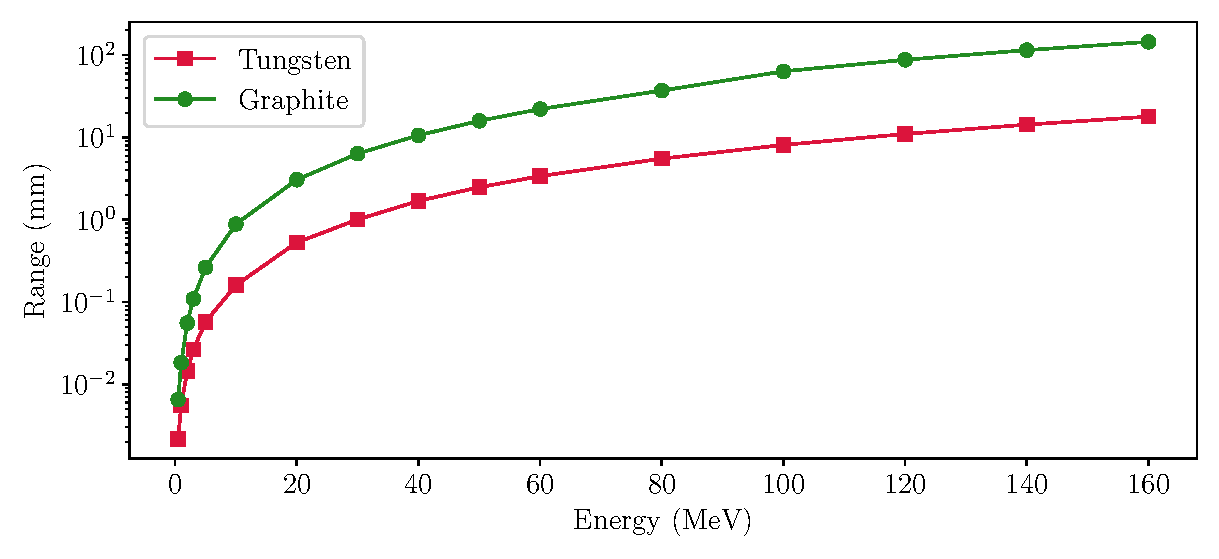
\includegraphics[width=0.9\columnwidth]{RangePlotLinac4/RangeL4.pdf}
    \caption{Range of particles as a function of incident ion energy.}
    \label{fig:RangeLinac4}
\end{figure}

From this figure, we can see how the range of the particles in the material increases as their energy increases. For the same energies, the particles have a much larger range in the case of graphite compared to tungsten. At LINAC4, the wires have a width of $40$ \si{\micro\metre} for the case of tungsten and 33 \si{\micro \metre} for the case of graphite wires. 

The range of protons is larger than the detector thickness in most of the energy range. Only tungsten detectors placed at energies smaller than 5  \si[]{\mega\electronvolt} are expected to get a positive charge deposition. The electrons in an \hm ion have energy much smaller than the proton. It is actually reduced a factor $m_p / m_e = 1836.15$ compared to the energy of the \hm ions.  Electrons are expected to deposit all their energy in all the SEM grids and Wire scanners at Linac4. So we expect to always have a double negative charge contribution. 

Table \ref{tab:ChargePar} summarizes the values for $\eta$ and $\mu$ parameters along the Linac4 accelerator range. This table also summarizes the values of the Backscattering probabilities for both electrons and protons. All these values have been calculated with Geant4 \parencite[][]{ref:Geant4}. The backscattering probability is negligible for the protons. Contrarily, electron backscattering probability is not negligible. In the case of tungsten, for ion energies of 160 MeV half of the electrons are backscattered.

% Please add the following required packages to your document preamble:
% \usepackage{multirow}
\begin{table}[h]
    \begin{tabular}{cccccccccc}
    \hline
    \multirow{2}{*}{\begin{tabular}[c]{@{}c@{}}$p^+$ energy \\ (MeV)\end{tabular}} & \multirow{2}{*}{\begin{tabular}[c]{@{}c@{}}$e^-$ energy\\ (keV)\end{tabular}} & \multicolumn{4}{c}{Graphite} & \multicolumn{4}{c}{Tungsten} \\ \cline{3-10}  &   & $\eta$   & $\mu$     & $BS_p$ & $BS_e$   & $\eta$ & $\mu$     & $BS_p$ & $BS_e$     \\ \hline
    3                                                                     & 1.63                                                                           & 0.001 & 0.918 & 0.0 & 0.081 & 1.0 & 0.632  & 0.0 & 0.367   \\
    50                                                                    & 27.23                                                                          & 0.0   & 0.931  & 0.0 & 0.068 & 0.0 & 0.506  & 0.0 & 0.493  \\
    102                                                                   & 55.55                                                                          & 0.0   & 0.887  & 0.0 & 0.112 & 0.0 & 0.487 & 0.0 & 0.512 \\
    160                                                                   & 87.14                                                                          & 0.0   & 0.857  & 0.0 & 0.142 & 0.0 & 0.464  & 0.0 & 0.536   \\ \hline
    \end{tabular}
    
    \caption{Summary of charge deposition and backscattering probabilities for Tungsten ($40 \mu m$) and Graphite ($33 \mu m$)} detectors.
    \label{tab:ChargePar}
\end{table}

Figure \ref{fig:SEYmat} shows the Secondary Emission yield calculated with the semiempirical Sternglass formula (Eq. \ref{eq:sey}) as a function of the incident proton energy.  In both materials, the SEY reaches a maximum ( $~ 0.1 $ MeV ) which is followed by a decrease in the SEY. Graphite presents a higher SEY at smaller proton energies whereas tungsten presents a higher SEY at higher incident particle eneriges. 

\begin{figure}[h]
    \centering
    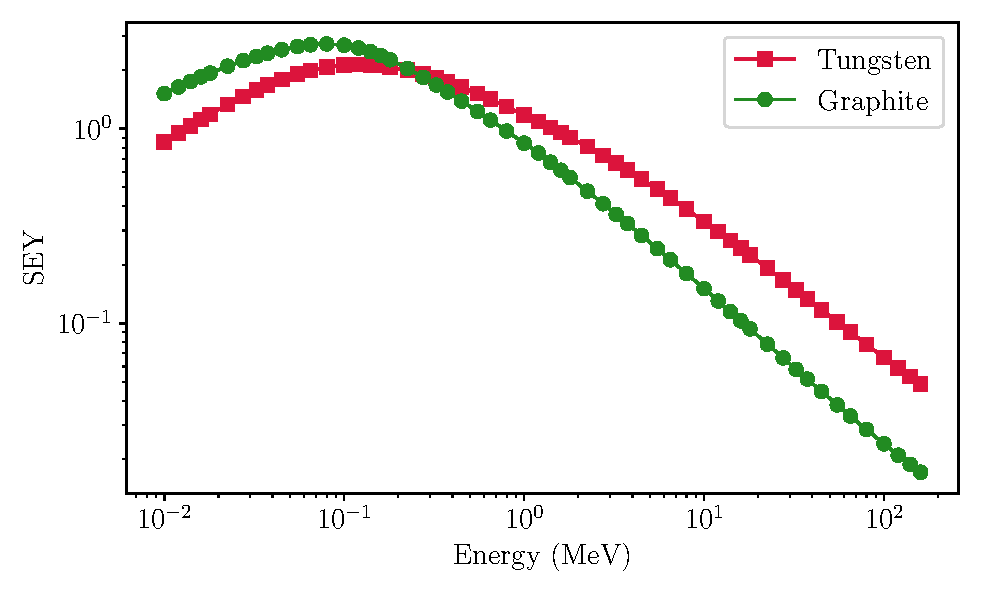
\includegraphics[width=0.85\columnwidth]{Figure_SEY/SEY_compa.pdf}
    \caption{Secondary Emission Yield as a function of incident proton energy. }
    \label{fig:SEYmat}
\end{figure}

As an example, figure \ref{fig:ProfComparison} shows a simulated beam profile at 3 MeV and 160 MeV. From these figures, we can observe how at 3 (MeV) the positive contribution to the charge is predominant for the case of tungsten wires while it remains negative in the case of graphite wires. Due to the smaller SEY of graphite at 160 (MeV), the absolute registered signal at this energy is higher than the one registered by the tungsten wires. 

\begin{figure}[h]
    \centering
    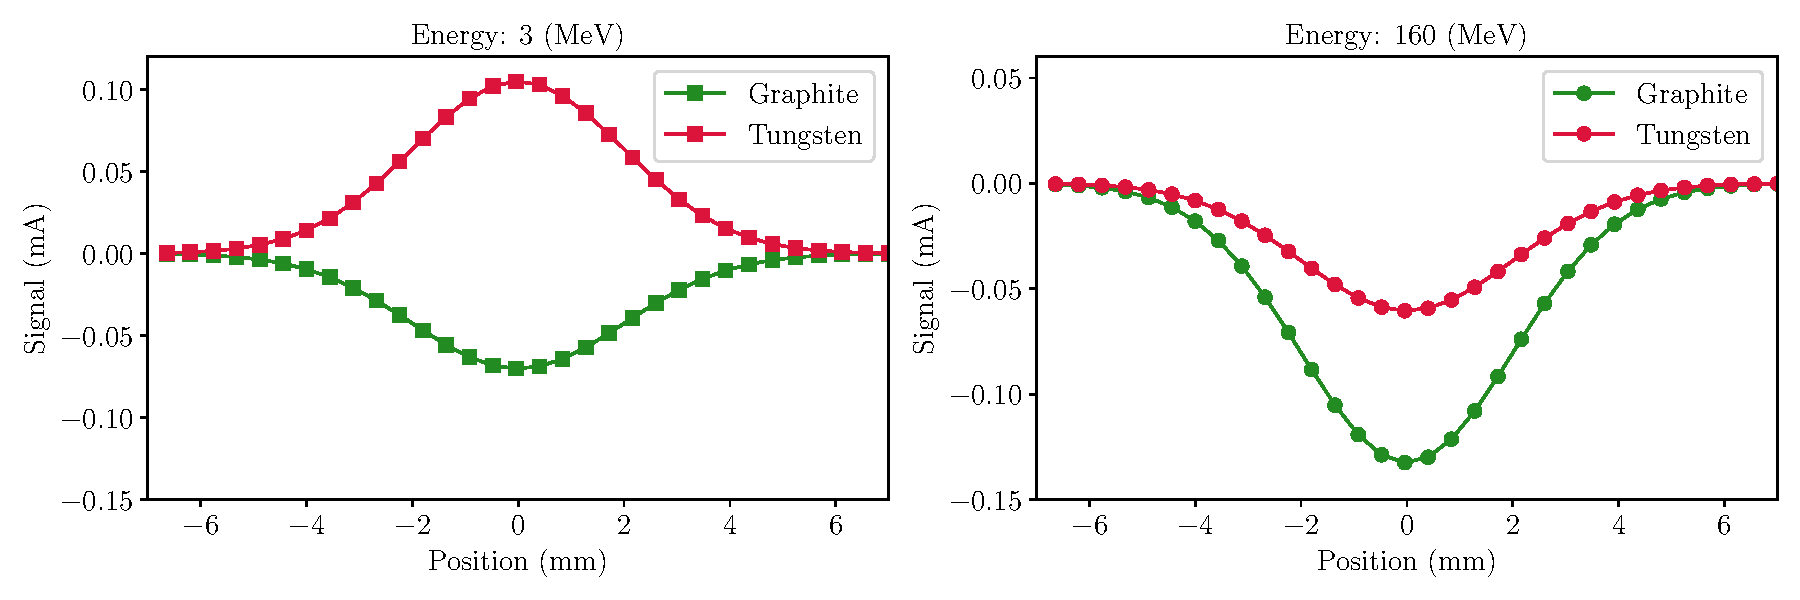
\includegraphics[width=0.85\columnwidth]{Figure_ProfCompa/ProfileComparison.pdf}
    \caption{Expected transverse beam profile for incident \hm particles. Left: 3 (MeV), Right: 160 (MeV). For these simulations, a 25 mA, 100 $\mu s$ particle beam was considered. }
    \label{fig:ProfComparison}
\end{figure}

At Linac4, even if these detectors are called Secondary Emission Monitors, the biggest contribution to the charge formation is the charge deposition term. To prevent misinterpretations, SE is typically suppressed by a bias current.  At LINAC4, the detectors at lower energies are usually conformed with graphite wires, to avoid the positive contribution of the proton charge deposition. 
